\documentclass[10pt]{standalone}
\usepackage{pgfplots}
\pgfplotsset{compat=1.15}
\usepackage{mathrsfs}
\usetikzlibrary{arrows}
\newcommand{\degre}{\ensuremath{^\circ}}
\pagestyle{empty}
\begin{document}
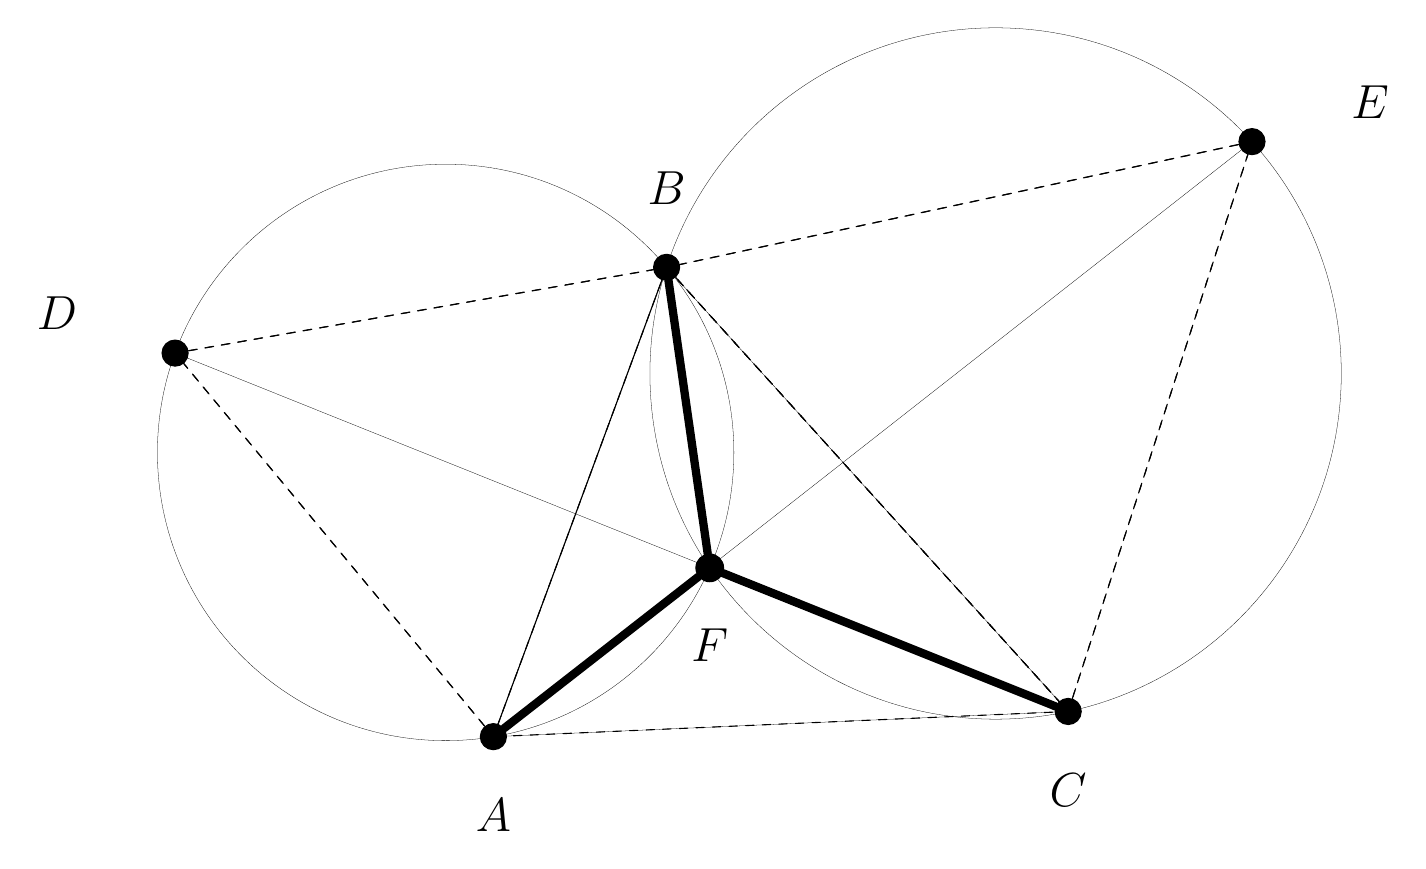
\begin{tikzpicture}[line cap=round,line join=round,x=1cm,y=1cm]

    \draw[dashed] (-4.1,4.05) -- (1,-1.59) -- (-6.3,-1.91) -- cycle;
    \draw[dashed] (-4.1,4.05) -- (-6.3,-1.91) -- (-10.342303152694532,2.961070905698067) -- cycle;
    \draw[dashed] (-4.1,4.05) -- (1,-1.59) -- (3.3343832773442346,5.646729559300637) -- cycle;


    \draw [line width=0.1pt] (0.07812775911474486,2.7022431864335457) circle (4.390125282950362cm);
    \draw [line width=0.1pt] (-6.906150549766938,1.6997871156857822) circle (3.6603253283764046cm);

    \draw (-6.3,-1.91) node[circle,draw, fill=black, minimum size=5pt] (A) [label={[yshift=-1.5cm]\LARGE$A$}] {};
    \draw (-4.1,4.05) node[circle,draw, fill=black, minimum size=5pt] (B) [label={[yshift=0.5cm]\LARGE$B$}] {};
    \draw (1,-1.59) node[circle,draw, fill=black, minimum size=5pt] (C) [label={[yshift=-1.5cm]\LARGE$C$}] {};
    \draw (-10.342303152694532,2.961070905698067) node[circle,draw, fill=black, minimum size=5pt] (D) [label={[xshift=-1.5cm]\LARGE$D$}] {};
    \draw (3.3343832773442346,5.646729559300637) node[circle,draw, fill=black, minimum size=5pt] (E) [label={[xshift=1.5cm]\LARGE$E$}] {};
    \draw (-3.5522491687374593,0.23372878264360902) node[circle,draw, fill=black, minimum size=10pt] (F) [label={[yshift=-1.5cm]\LARGE$F$}] {};

    % Original triangle
    \draw[ultra thin] (B)-- (C);
    \draw[ultra thin] (C)-- (A);
    \draw[ultra thin] (A)-- (B);
    % Equilateral triangles
    \draw[dashed] (B) -- (A);
    \draw[dashed] (A) -- (D);
    \draw[dashed] (D) -- (B);
    \draw[dashed] (B) -- (C);
    \draw[dashed] (C) -- (E);
    \draw[dashed] (E) -- (B);
    % Steiner edges
    \draw [line width=3pt] (F)-- (A);
    \draw [line width=3pt] (F)-- (B);
    \draw [line width=3pt] (F)-- (C);
    % Simson lines
    \draw[ultra thin] (D) -- (C);
    \draw[ultra thin] (E) -- (A);
\end{tikzpicture}
\end{document}